\section{Osnovni geometrijski pojmi}

            
                Evklid je v prvi knjigi \textit{Elementov} postavil $23$ 'opredelitev' temeljnih geometrijskih pojmov.
                Med njimi so:
                \begin{itemize}
                    \item \textbf{Točka} je tisto, kar nima delov -- nima razsežnosti.
                    \item \textbf{Črta} je dolžina brez širine -- ena razsežnost.
                    \item \textbf{Ploskev} je tisto, kar ima samo dolžino in širino -- dve razsežnosti.
                \end{itemize}
            

            
                Tem trditvam sledijo \textbf{aksiomi} (temeljne resnice) -- privzamemo jih kot veljavne hipoteze,
                 \textbf{izreki}~-- dokazujemo jih z aksiomi in prej dokazanimi izreki, 
                 in \textbf{definicije} -- opisi novih pojmov in lastnosti.
            
        

        
            \subsection{Incidenčni aksiomi}

            \begin{definicija}
                \textit{Incidenca} je relacija, ki povezuje točko in premico -- premica in točka sta v relaciji,
                 če točka leži na premici; $A~R~p$, če $A\in p$.
            \end{definicija}

            \begin{aksiom}
                Za dve različni točki $A$ in $B$ obstaja natanko določena premica $p$, tako da točki $A$ in $B$ ležita na njej.
            \end{aksiom}

            \begin{aksiom}
                Za vsako premico $p$ obstajata vsaj dve različni točki $P$ in $Q$, ki ležita na njej.
            \end{aksiom}

            \begin{aksiom}
                Obstajajo tri različne točke, ki ne ležijo hkrati na isti premici.
            \end{aksiom}
        


        
            \begin{definicija}
                Točke $A_1, A_2, A_3, \dots$, ki ležijo na isti premici, so \textbf{kolinearne}, 
                če ne ležijo na isti premici, pa so \textbf{nekolinearne}.
            \end{definicija}

            \begin{izrek}
                Dve različni premici imata lahko največ eno skupno točko.
            \end{izrek}

            \begin{definicija}
                Premici, ki imata natanko eno skupno točko, se \textbf{sekata}, imenujemo ju \textbf{sečnici},
                njuno skupno točko pa \textbf{presečišče} premic.
            \end{definicija}

            \begin{definicija}
                Premici, ki ležita na isti ravnini in nimata nobene skupne točke ali imata vse točke skupne -- sovpadata, sta \textbf{vzporedni}, imenujemo ju \textbf{vzporednici}.
            \end{definicija}
        


        
            \begin{aksiom}
                Če so tri različne točke kolinearne, ena vedno leži med drugima dvema.

                \begin{figure}[H]
                    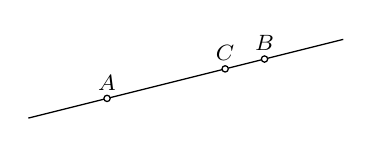
\begin{tikzpicture}
                        % \clip (0,0) rectangle (14.000000,10.000000);
                        {\footnotesize

                        % Drawing line A B
                        \draw [line width=0.016cm] (1.000000,1.250000) -- (1.961194,1.490299);%
                        \draw [line width=0.016cm] (2.038806,1.509701) -- (3.461194,1.865299);%
                        \draw [line width=0.016cm] (3.538806,1.884701) -- (3.961194,1.990299);%
                        \draw [line width=0.016cm] (4.038806,2.009701) -- (5.000000,2.250000);%

                        % Marking point A by circle
                        \draw [line width=0.016cm] (2.000000,1.500000) circle (0.040000);%
                        \draw (2.000000,1.500000) node [anchor=south] { $A$ };%

                        % Marking point C by circle
                        \draw [line width=0.016cm] (3.500000,1.875000) circle (0.040000);%
                        \draw (3.500000,1.875000) node [anchor=south] { $C$ };%

                        % Marking point B by circle
                        \draw [line width=0.016cm] (4.000000,2.000000) circle (0.040000);%
                        \draw (4.000000,2.000000) node [anchor=south] { $B$ };%
                        }
                    \end{tikzpicture}
                \end{figure}
            \end{aksiom}

            \begin{aksiom}
                Če sta $A$ in $B$ različni točki premice $p$, potem na premici $p$ ležita vsaj še točki $C$ in $D$,
                in sicer $C$ leži med $A$ in $B$, $D$ pa tako, da je $C$ med $A$ in $D$.

                \begin{figure}[H]
                    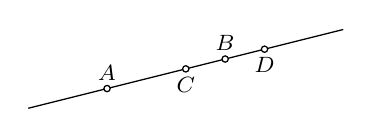
\begin{tikzpicture}
                        % \clip (0,0) rectangle (14.000000,10.000000);
                        {\footnotesize

                        % Drawing line A B
                        \draw [line width=0.016cm] (1.000000,1.250000) -- (1.961194,1.490299);%
                        \draw [line width=0.016cm] (2.038806,1.509701) -- (2.961194,1.740299);%
                        \draw [line width=0.016cm] (3.038806,1.759701) -- (3.461194,1.865299);%
                        \draw [line width=0.016cm] (3.538806,1.884701) -- (3.961194,1.990299);%
                        \draw [line width=0.016cm] (4.038806,2.009701) -- (5.000000,2.250000);%

                        % Marking point A by circle
                        \draw [line width=0.016cm] (2.000000,1.500000) circle (0.040000);%
                        \draw (2.000000,1.500000) node [anchor=south] { $A$ };%

                        % Marking point C by circle
                        \draw [line width=0.016cm] (3.000000,1.750000) circle (0.040000);%
                        \draw (3.000000,1.750000) node [anchor=north] { $C$ };%

                        % Marking point B by circle
                        \draw [line width=0.016cm] (3.500000,1.875000) circle (0.040000);%
                        \draw (3.500000,1.875000) node [anchor=south] { $B$ };%

                        % Marking point D by circle
                        \draw [line width=0.016cm] (4.000000,2.000000) circle (0.040000);%
                        \draw (4.000000,2.000000) node [anchor=north] { $D$ };%
                        }
                    \end{tikzpicture}
                \end{figure}
            \end{aksiom}

            \begin{izrek}
                Med dvema različnima točkama premice je neskončno mnogo točk.
            \end{izrek}

        
        

        
            \begin{definicija}
                Množica točk premice, ki ležijo med različnima točkama $A$ in $B$, vključno z $A$ in $B$,
                je \textbf{daljica~$AB$}. Točki $A$ in $B$ sta njeni \textbf{krajišči}.

                \begin{figure}[H]
                    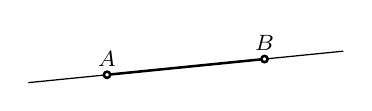
\begin{tikzpicture}
                        % \clip (0,0) rectangle (14.000000,10.000000);
                        {\footnotesize

                        % Drawing line A B
                        \draw [line width=0.016cm] (1.000000,1.400000) -- (1.960199,1.496020);%
                        \draw [line width=0.016cm] (2.039801,1.503980) -- (3.960199,1.696020);%
                        \draw [line width=0.016cm] (4.039801,1.703980) -- (5.000000,1.800000);%

                        % Drawing segment A B
                        \draw [line width=0.032cm] (2.039801,1.503980) -- (3.960199,1.696020);%

                        % Marking point A by circle
                        \draw [line width=0.032cm] (2.000000,1.500000) circle (0.040000);%
                        \draw (2.000000,1.500000) node [anchor=south] { $A$ };%

                        % Marking point B by circle
                        \draw [line width=0.032cm] (4.000000,1.700000) circle (0.040000);%
                        \draw (4.000000,1.700000) node [anchor=south] { $B$ };%
                        }
                    \end{tikzpicture}
                \end{figure}
            \end{definicija}

            \begin{definicija}
                Poljubna točka premice razdeli premico na dva \textbf{poltraka}. To točko imenujemo \textbf{izhodišče}, ponavadi jo označimo z $O$.

                \begin{figure}[H]
                    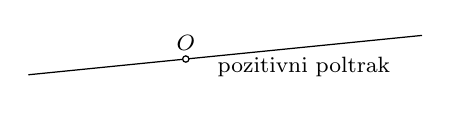
\begin{tikzpicture}
                        % \clip (0,0) rectangle (14.000000,10.000000);
                        {\footnotesize

                        % Drawing line O B
                        \draw [line width=0.016cm] (1.000000,1.300000) -- (2.960199,1.496020);%
                        \draw [line width=0.016cm] (3.039801,1.503980) -- (6.000000,1.800000);%

                        % Marking point O by circle
                        \draw [line width=0.016cm] (3.000000,1.500000) circle (0.040000);%
                        \draw (3.000000,1.500000) node [anchor=south] { $O$ };%

                        % Marking point poz
                        \draw (4.500000,1.400000) node  {pozitivni poltrak };%
                        }
                    \end{tikzpicture}
                \end{figure}
            \end{definicija}

            \begin{definicija}
                Premica, na kateri leži daljica oziroma poltrak, je \textbf{nosilka} daljice oziroma poltraka.
            \end{definicija}
        


        
            \begin{definicija}
                \textbf{Enostavni lik} je množica točk v ravnini, ki jo omejuje sklenjena krivulja, ki sama sebe ne seka.
            \end{definicija}

            \begin{definicija}

                Množica točk v ravnini je \textbf{konveksna}, če za poljubni točki $A$ in $B$ iz te množice velja, da je daljica $AB$ njena podmnožica.
                $$ \mathcal{M}\text{~konveksna} \Leftrightarrow \forall A, B\in\mathcal{M}\Rightarrow AB\subseteq\mathcal{M} $$
                Množica točk, ki ni konveksna, je \textbf{nekonveksna} oziroma \textbf{konkavna}.
                $$ \mathcal{M}\text{~nekonveksna} \Leftrightarrow \exists A, B\in\mathcal{M}\Rightarrow AB\not\subset\mathcal{M} $$
            
                \begin{figure}[H]
                    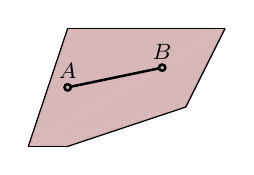
\begin{tikzpicture}
                        % \clip (0,0) rectangle (14.000000,10.000000);
                        {\footnotesize

                        % Changing color 215 183 183
                        \definecolor{r215g183b183}{rgb}{0.843137,0.717647,0.717647}%
                        \color{r215g183b183}% 

                        % Filling triangle C D E
                        \fill (1.500000,1.500000) -- (2.000000,1.500000) -- (3.500000,2.000000);%

                        % Filling triangle C E F
                        \fill (1.500000,1.500000) -- (3.500000,2.000000) -- (4.000000,3.000000);%

                        % Filling triangle C F G
                        \fill (1.500000,1.500000) -- (4.000000,3.000000) -- (2.000000,3.000000);%

                        % Changing color 0 0 0
                        \definecolor{r0g0b0}{rgb}{0.000000,0.000000,0.000000}%
                        \color{r0g0b0}% 

                        % Drawing segment C D
                        \draw [line width=0.016cm] (1.500000,1.500000) -- (2.000000,1.500000);%

                        % Drawing segment D E
                        \draw [line width=0.016cm] (2.000000,1.500000) -- (3.500000,2.000000);%

                        % Drawing segment E F
                        \draw [line width=0.016cm] (3.500000,2.000000) -- (4.000000,3.000000);%

                        % Drawing segment F G
                        \draw [line width=0.016cm] (4.000000,3.000000) -- (2.000000,3.000000);%

                        % Drawing segment G C
                        \draw [line width=0.016cm] (2.000000,3.000000) -- (1.500000,1.500000);%

                        % Marking point A by circle
                        \draw [line width=0.032cm] (2.000000,2.250000) circle (0.040000);%
                        \draw (2.000000,2.250000) node [anchor=south] { $A$ };%

                        % Marking point B by circle
                        \draw [line width=0.032cm] (3.200000,2.500000) circle (0.040000);%
                        \draw (3.200000,2.500000) node [anchor=south] { $B$ };%

                        % Drawing segment A B
                        \draw [line width=0.032cm] (2.039159,2.258158) -- (3.160841,2.491842);%
                        \color{black}
                        }
                    \end{tikzpicture}
                \end{figure}

                \begin{figure}[H]
                    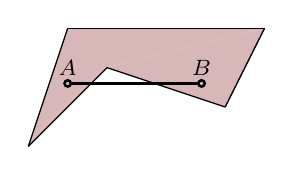
\begin{tikzpicture}
                        % \clip (0,0) rectangle (14.000000,10.000000);
                        {\footnotesize

                        % Changing color 215 183 183
                        \definecolor{r215g183b183}{rgb}{0.843137,0.717647,0.717647}%
                        \color{r215g183b183}% 

                        % Filling triangle C D G
                        \fill (1.500000,1.500000) -- (2.500000,2.500000) -- (2.000000,3.000000);%

                        % Filling triangle D E F
                        \fill (2.500000,2.500000) -- (4.000000,2.000000) -- (4.500000,3.000000);%

                        % Filling triangle D F G
                        \fill (2.500000,2.500000) -- (4.500000,3.000000) -- (2.000000,3.000000);%

                        % Changing color 0 0 0
                        \definecolor{r0g0b0}{rgb}{0.000000,0.000000,0.000000}%
                        \color{r0g0b0}% 

                        % Drawing segment C D
                        \draw [line width=0.016cm] (1.500000,1.500000) -- (2.500000,2.500000);%

                        % Drawing segment D E
                        \draw [line width=0.016cm] (2.500000,2.500000) -- (4.000000,2.000000);%

                        % Drawing segment E F
                        \draw [line width=0.016cm] (4.000000,2.000000) -- (4.500000,3.000000);%

                        % Drawing segment F G
                        \draw [line width=0.016cm] (4.500000,3.000000) -- (2.000000,3.000000);%

                        % Drawing segment G C
                        \draw [line width=0.016cm] (2.000000,3.000000) -- (1.500000,1.500000);%

                        % Marking point A by circle
                        \draw [line width=0.032cm] (2.000000,2.300000) circle (0.040000);%
                        \draw (2.000000,2.300000) node [anchor=south] { $A$ };%

                        % Marking point B by circle
                        \draw [line width=0.032cm] (3.700000,2.300000) circle (0.040000);%
                        \draw (3.700000,2.300000) node [anchor=south] { $B$ };%

                        % Drawing segment A B
                        \draw [line width=0.032cm] (2.040000,2.300000) -- (3.660000,2.300000);%
                        \color{black}
                        }
                    \end{tikzpicture}
                \end{figure}

            \end{definicija}
        


        
            \begin{definicija}
                Dva poltraka s skupnim izhodiščem določata dva \textbf{kota}.
                Izhodišče poltrakov imenujemo \textbf{vrh} kota, poltraka pa imenujemo \textbf{kraka} kota.
                
                \begin{figure}[H]
                    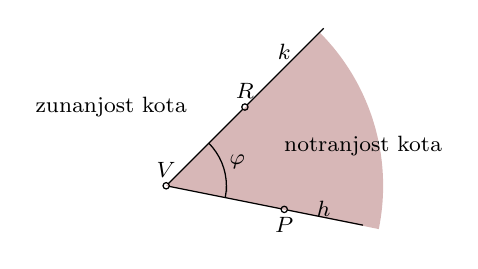
\begin{tikzpicture}
                        % \clip (0,0) rectangle (14.000000,10.000000);
                        {\footnotesize

                        % Changing color 215 183 183
                        \definecolor{r215g183b183}{rgb}{0.843137,0.717647,0.717647}%
                        \color{r215g183b183}% 

                        % Filling circle arc V B 56.31
                        \fill (2.500000,2.500000) -- (5.200000,1.949999) -- (5.204824,1.974235) arc (349:360:2.755449 and 2.755449) --(5.255449,2.500000) arc (0:44:2.755449 and 2.755449) -- (4.455318,4.441451) -- cycle;%

                        % Changing color 0 0 0
                        \definecolor{r0g0b0}{rgb}{0.000000,0.000000,0.000000}%
                        \color{r0g0b0}% 

                        % Drawing line V P
                        % \draw [line width=0.016cm] (1.000000,2.800000) -- (2.460777,2.507845);%
                        \draw [line width=0.016cm] (2.539223,2.492155) -- (3.960777,2.207845);%
                        \draw [line width=0.016cm] (4.039223,2.192155) -- (5.000000,2.000000);%

                        % Drawing line V R
                        % \draw [line width=0.016cm] (1.000000,1.000000) -- (2.471716,2.471716);%
                        \draw [line width=0.016cm] (2.528284,2.528284) -- (3.471716,3.471716);%
                        \draw [line width=0.016cm] (3.528284,3.528284) -- (4.500000,4.500000);%

                        % Marking point V by circle
                        \draw [line width=0.016cm] (2.500000,2.500000) circle (0.040000);%
                        \draw (2.500000,2.500000) node [anchor=south] { $V$ };%

                        % Marking point P by circle
                        \draw [line width=0.016cm] (4.000000,2.200000) circle (0.040000);%
                        \draw (4.000000,2.200000) node [anchor=north] { $P$ };%

                        % Marking point R by circle
                        \draw [line width=0.016cm] (3.500000,3.500000) circle (0.040000);%
                        \draw (3.500000,3.500000) node [anchor=south] { $R$ };%

                        % Marking point h
                        \draw (4.500000,2.000000) node [anchor=south] { $h$ };%

                        % Marking point k
                        \draw (4.000000,4.000000) node [anchor=south] { $k$ };%

                        % Drawing arc V A 56.31
                        \draw [line width=0.016cm] (3.250000,2.350000) -- (3.250800,2.354059) arc (349:360:0.764853 and 0.764853) --(3.264853,2.500000) arc (0:45:0.764853 and 0.764853);%

                        % Marking point \varphi
                        \draw (3.200000,2.800000) node [anchor=west] { $\varphi$ };%

                        % Marking point zun
                        \draw (1.800000,3.500000) node  { zunanjost kota };%

                        % Marking point not
                        \draw (5.000000,3.000000) node  { notranjost kota };%
                        \color{black}
                        }
                    \end{tikzpicture}
                \end{figure}
            \end{definicija}

            
                Če poltraka ne ležita na isti premici, je eden od kotov konveksen, drugi pa je nekonveksen.
            

            
                Kot lahko označimo na več načinov:
                \begin{itemize}
                    \item $\angle(h,k)$, kjer sta $h$ in $k$ poltraka, ki kot določata;
                    \item $\angle PVR$, kjer je $P$ točka na enem poltraku, $V$ vrh kota in $R$ točka na drugem poltraku;
                    \item $\alpha, \beta, \gamma, \dots$ -- z grškimi črkami.
                \end{itemize}
            
        


        
            \begin{definicija}
                Če poltraka s skupnim izhodiščem ležita na isti premici, vendar na različnih straneh izhodišča,
                določata dva enaka konveksna kota -- \textbf{iztegnjena kota}.

                \begin{figure}[H]
                    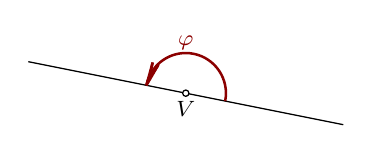
\begin{tikzpicture}
                        % \clip (0,0) rectangle (14.000000,10.000000);
                        {\footnotesize

                        % Drawing line V h
                        \draw [line width=0.016cm] (1.000000,2.000000) -- (2.960777,1.607845);%
                        \draw [line width=0.016cm] (3.039223,1.592155) -- (5.000000,1.200000);%

                        % Marking point V by circle
                        \draw [line width=0.016cm] (3.000000,1.600000) circle (0.040000);%
                        \draw (3.000000,1.600000) node [anchor=north] { $V$ };%

                        % Changing color 139 0 0
                        \definecolor{r139g0b0}{rgb}{0.545098,0.000000,0.000000}%
                        \color{r139g0b0}% 

                        % Drawing arc V h 180.00
                        \draw [line width=0.032cm] (3.500000,1.500000) -- (3.500534,1.502706) arc (349:360:0.509902 and 0.509902) --(3.509902,1.600000) arc (0:168:0.509902 and 0.509902) -- (2.500000,1.700000);%

                        % Marking point \varphi
                        \draw (3.000000,2.050000) node [anchor=south] { $\varphi$ };%

                        % Drawing arrow C A 1.00
                        \draw [line width=0.032cm] (2.651137,1.959148) -- (2.500000,1.700000);%
                        \draw [line width=0.032cm] (2.651137,1.959148) -- (2.538342,1.791430);%
                        \draw [line width=0.032cm] (2.578914,1.989435) -- (2.500000,1.700000);%
                        \draw [line width=0.032cm] (2.578914,1.989435) -- (2.538342,1.791430);%
                        \color{black}
                        }
                    \end{tikzpicture}
                \end{figure}
            \end{definicija}

            \begin{definicija}
                Če se poltraka na isti premici prekrivata, določata \textbf{polni kot} ali \textbf{ničelni kot}.

                \begin{figure}[H]
                    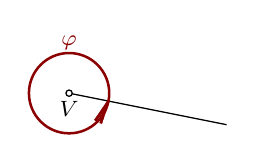
\begin{tikzpicture}
                        % \clip (0,0) rectangle (14.000000,10.000000);
                        {\footnotesize

                        % Drawing line V h
                        % \draw [line width=0.016cm] (1.000000,2.000000) -- (2.960777,1.607845);%
                        \draw [line width=0.016cm] (3.039223,1.592155) -- (5.000000,1.200000);%

                        % Marking point V by circle
                        \draw [line width=0.016cm] (3.000000,1.600000) circle (0.040000);%
                        \draw (3.000000,1.600000) node [anchor=north] { $V$ };%

                        % Changing color 139 0 0
                        \definecolor{r139g0b0}{rgb}{0.545098,0.000000,0.000000}%
                        \color{r139g0b0}% 

                        % Drawing arc V h 360.00
                        \draw [line width=0.032cm] (3.000000,1.600000) circle (0.509902);%

                        % Marking point \varphi
                        \draw (3.000000,2.050000) node [anchor=south] { $\varphi$ };%

                        % Drawing arrow k h 1.00
                        \draw [line width=0.032cm] (3.331960,1.251479) -- (3.500000,1.500000);%
                        \draw [line width=0.032cm] (3.331960,1.251479) -- (3.455661,1.411322);%
                        \draw [line width=0.032cm] (3.402008,1.216456) -- (3.500000,1.500000);%
                        \draw [line width=0.032cm] (3.402008,1.216456) -- (3.455661,1.411322);%
                        \color{black}
                        }
                    \end{tikzpicture} ~~~~~
                    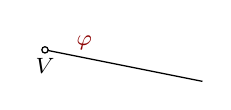
\begin{tikzpicture}
                        % \clip (0,0) rectangle (14.000000,10.000000);
                        {\footnotesize

                        % Drawing line V h
                        % \draw [line width=0.016cm] (1.000000,2.000000) -- (2.960777,1.607845);%
                        \draw [line width=0.016cm] (3.039223,1.592155) -- (5.000000,1.200000);%

                        % Marking point V by circle
                        \draw [line width=0.016cm] (3.000000,1.600000) circle (0.040000);%
                        \draw (3.000000,1.600000) node [anchor=north] { $V$ };%

                        % Changing color 139 0 0
                        \definecolor{r139g0b0}{rgb}{0.545098,0.000000,0.000000}%
                        \color{r139g0b0}% 

                        % Marking point \varphi
                        \draw (3.500000,1.500000) node [anchor=south] { $\varphi$ };%
                        \color{black}
                        }
                    \end{tikzpicture}
                \end{figure}

            \end{definicija}
        


        
            \begin{definicija}
                Kota s skupnim vrhom, ki imata en skupen krak, presek njunih notranjosti pa je prazen, sta \textbf{sosedna kota}.

                \begin{figure}[H]
                    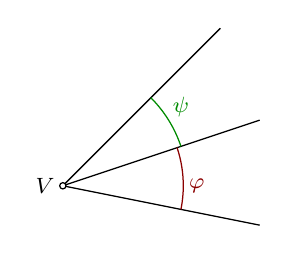
\begin{tikzpicture}
                        % \clip (0,0) rectangle (14.000000,10.000000);
                        {\footnotesize

                        % Drawing line V P
                        \draw [line width=0.016cm] (4.000000,1.000000) -- (1.539223,1.492155);%
                        % \draw [line width=0.016cm] (1.460777,1.507845) -- (1.000000,1.600000);%

                        % Drawing line V Q
                        % \draw [line width=0.016cm] (1.000000,1.333333) -- (1.462053,1.487351);%
                        \draw [line width=0.016cm] (1.537947,1.512649) -- (4.000000,2.333333);%

                        % Drawing line V R
                        % \draw [line width=0.016cm] (1.000000,1.000000) -- (1.471716,1.471716);%
                        \draw [line width=0.016cm] (1.528284,1.528284) -- (3.500000,3.500000);%

                        % Marking point V by circle
                        \draw [line width=0.016cm] (1.500000,1.500000) circle (0.040000);%
                        \draw (1.500000,1.500000) node [anchor=east] { $V$ };%

                        % Changing color 139 0 0
                        \definecolor{r139g0b0}{rgb}{0.545098,0.000000,0.000000}%
                        \color{r139g0b0}% 

                        % Drawing arc V P 29.74
                        \draw [line width=0.016cm] (3.000000,1.200000) -- (3.001601,1.208118) arc (349:360:1.529706 and 1.529706) --(3.029706,1.500000) arc (0:18:1.529706 and 1.529706) -- (2.951206,1.983735);%

                        % Marking point \varphi
                        \draw (3.200000,1.500000) node  { $\varphi$ };%

                        % Changing color 0 139 0
                        \definecolor{r0g139b0}{rgb}{0.000000,0.545098,0.000000}%
                        \color{r0g139b0}% 

                        % Drawing arc V Q 26.57
                        \draw [line width=0.016cm] (3.000000,2.000000) -- (2.994996,2.014768) arc (19:45:1.581139 and 1.581139);%

                        % Marking point \psi
                        \draw (3.000000,2.500000) node  { $\psi$ };%
                        \color{black}
                        }
                    \end{tikzpicture}
                \end{figure}
            \end{definicija}

            \begin{definicija}
                Sosedna kota, katerih kraka, ki  nista skupna, ležita na isti premici, sta \textbf{sokota}.
                
                \begin{figure}[H]
                    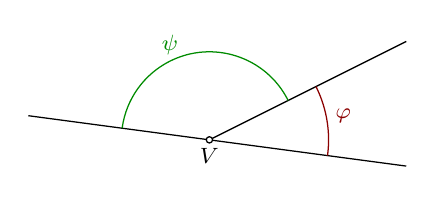
\begin{tikzpicture}
                        % \clip (0,0) rectangle (14.000000,10.000000);
                        {\footnotesize

                        % Drawing line V P
                        \draw [line width=0.016cm] (1.200000,1.806667) -- (3.460351,1.505287);%
                        \draw [line width=0.016cm] (3.539649,1.494713) -- (6.000000,1.166667);%

                        % Drawing line V Q
                        % \draw [line width=0.016cm] (2.700000,1.100000) -- (3.464223,1.482111);%
                        \draw [line width=0.016cm] (3.535777,1.517889) -- (6.000000,2.750000);%

                        % Marking point V by circle
                        \draw [line width=0.016cm] (3.500000,1.500000) circle (0.040000);%
                        \draw (3.500000,1.500000) node [anchor=north] { $V$ };%

                        % Changing color 139 0 0
                        \definecolor{r139g0b0}{rgb}{0.545098,0.000000,0.000000}%
                        \color{r139g0b0}% 

                        % Drawing arc V P 34.16
                        \draw [line width=0.016cm] (5.000000,1.300000) -- (5.001995,1.315578) arc (353:360:1.513275 and 1.513275) --(5.013275,1.500000) arc (0:26:1.513275 and 1.513275) -- (4.853514,2.176757);%

                        % Marking point \varphi
                        \draw (5.200000,1.800000) node  { $\varphi$ };%

                        % Changing color 0 139 0
                        \definecolor{r0g139b0}{rgb}{0.000000,0.545098,0.000000}%
                        \color{r0g139b0}% 

                        % Drawing arc V Q 145.84
                        \draw [line width=0.016cm] (4.500000,2.000000) -- (4.496176,2.007577) arc (27:172:1.118034 and 1.118034) -- (2.391774,1.647764);%

                        % Marking point \psi
                        \draw (3.000000,2.700000) node  { $\psi$ };%
                        \color{black}
                        }
                    \end{tikzpicture}
                \end{figure}
            \end{definicija}

        


        
            \begin{definicija}
                Tri nekolinearne točke $A$, $B$ in $C$ določajo \textbf{trikotnik} $\triangle ABC$.
                Točke $A$, $B$ in $C$ so \textbf{oglišča} trikotnika, daljice $AB$, $BC$ in $AC$ so njegove \textbf{stranice}.

            \begin{figure}
                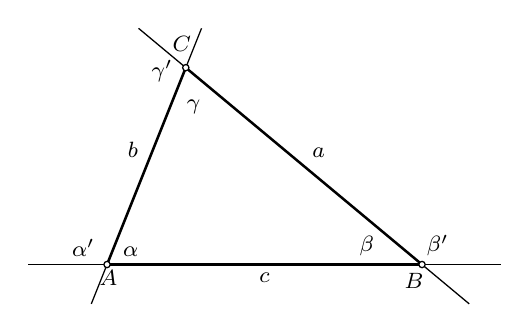
\begin{tikzpicture}
                    % \clip (0,0) rectangle (14.000000,10.000000);
                    {\footnotesize
                    
                    % Marking point A by circle
                    \draw [line width=0.016cm] (2.000000,1.500000) circle (0.040000);%
                    \draw (1.800000,1.530000) node [anchor=north west] { $A$ };%
                    
                    % Marking point B by circle
                    \draw [line width=0.016cm] (6.000000,1.500000) circle (0.040000);%
                    \draw (5.900000,1.500000) node [anchor=north] { $B$ };%
                    
                    % Marking point C by circle
                    \draw [line width=0.016cm] (3.000000,4.000000) circle (0.040000);%
                    \draw (2.950000,4.100000) node [anchor=south] { $C$ };%
                    
                    % Drawing line A B
                    \draw [line width=0.016cm] (1.000000,1.500000) -- (1.960000,1.500000);%
                    \draw [line width=0.016cm] (2.040000,1.500000) -- (5.960000,1.500000);%
                    \draw [line width=0.016cm] (6.040000,1.500000) -- (7.000000,1.500000);%
                    
                    % Drawing line B C
                    \draw [line width=0.016cm] (6.600000,1.000000) -- (6.030729,1.474393);%
                    \draw [line width=0.016cm] (5.969271,1.525607) -- (3.030729,3.974393);%
                    \draw [line width=0.016cm] (2.969271,4.025607) -- (2.400000,4.500000);%
                    
                    % Drawing line A C
                    \draw [line width=0.016cm] (1.800000,1.000000) -- (1.985144,1.462861);%
                    \draw [line width=0.016cm] (2.014856,1.537139) -- (2.985144,3.962861);%
                    \draw [line width=0.016cm] (3.014856,4.037139) -- (3.200000,4.500000);%
                    
                    % Marking point c
                    \draw (4.000000,1.500000) node [anchor=north] { $c$ };%
                    
                    % Marking point a
                    \draw (4.500000,2.750000) node [anchor=south west] { $a$ };%
                    
                    % Marking point b
                    \draw (2.500000,2.750000) node [anchor=south east] { $b$ };%
                    
                    % Marking point \gamma
                    \draw (3.100000,3.700000) node [anchor=north] { $\gamma$ };%
                    
                    % Marking point \gamma'
                    \draw (2.700000,4.200000) node [anchor=north] { $\gamma'$ };%
                    
                    % Marking point \beta
                    \draw (5.300000,1.500000) node [anchor=south] { $\beta$ };%
                    
                    % Marking point \beta'
                    \draw (6.200000,1.500000) node [anchor=south] { $\beta'$ };%
                    
                    % Marking point \alpha
                    \draw (2.300000,1.500000) node [anchor=south] { $\alpha$ };%
                    
                    % Marking point \alpha'
                    \draw (1.700000,1.500000) node [anchor=south] { $\alpha'$ };%
                    
                    % Drawing segment A B
                    \draw [line width=0.032cm] (2.040000,1.500000) -- (5.960000,1.500000);%
                    
                    % Drawing segment B C
                    \draw [line width=0.032cm] (5.969271,1.525607) -- (3.030729,3.974393);%
                    
                    % Drawing segment A C
                    \draw [line width=0.032cm] (2.014856,1.537139) -- (2.985144,3.962861);%
                    }
                \end{tikzpicture}
            \end{figure}

                Koti $\alpha$, $\beta$ in $\gamma$ so \textbf{notranji koti}, 
                njihovi sokoti $\alpha'$, $\beta'$ in $\gamma'$ pa so \textbf{zunanji koti} trikotnika.

            \end{definicija}

            
                Trikotnik je \textbf{pozitivno orientiran}, če si njegova oglišča sledijo v nasprotni smeri vrtenja urinega kazalca; 
                če si sledijo v smeri vrtenja urinega kazalca, pa je \textbf{negativno orientiran}.
            
        


        
            \begin{definicija}
                Točke $A_1, A_2, A_3, \dots, A_n$ v ravnini, od katerih nobene zaporedne tri niso kolinearne, določajo \textbf{$n$-kotnik}.

                Točke $A_1, A_2, A_3, \dots, A_n$ so \textbf{oglišča} $n$-kotnika;
                daljice, ki povezujejo sosedni oglišči, $A_1A_2, A_2A_3, \dots, A_nA_1$ so \textbf{stranice} $n$-kotnika;
                daljice, ki povezujejo po dve nesosedni oglišči, pa so \textbf{diagonale} $n$-kotnika.
            \end{definicija}

            
                Poljuben $n$-kotnika ima $$\dfrac{n(n-3)}{2}$$ diagonal -- iz vsakega od $n$ oglišč gre $n-3$ diagonal, vsaka pa je šteta dvakrat.
            

            
                Če za vsako nosilko stranice $n$-kotnika velja, da preostala oglišča ležijo na isti strani te nosilke, je $n$-kotnik \textbf{konveksen}.
            
        




        %%%%% naloge

        ~\\~\\

            \begin{naloga}
                Izračunajte število diagonal: $17$-kotnika, $31$-kotnika in $28$-kotnika.                
            \end{naloga}

            \begin{naloga}
                Ugotovite, ali obstaja $n$-kotnik, ki ima desetino toliko diagonal kot $28$-kotnik.
                Če obstaja, izračunajte, koliko stranic ima.
            \end{naloga}   
            
            \begin{naloga}
                Kateri $n$-kotnik ima štirikrat toliko diagonal kot stranic?
            \end{naloga}
        
            \begin{naloga}
                Izračunajte, kateri $n$-kotnik ima: $104$ diagonale, $230$ diagonal, $2n-5$ diagonal.
            \end{naloga}

            \begin{naloga}
                Pokažite, da ne obstaja $n$-kotnik, ki ima $13$ diagonal.  
            \end{naloga}
            

            \begin{naloga}
                Za vsako od spodnjih izjav ugotovite, ali je pravilna ali nepravilna.
                \begin{itemize}
                    \item Tri različne točke, so vedno nekolinearne.
                    \item Petkotnik ima enako število diagonal in stranic.
                    \item Štiri različne premice se sekajo v največ $4$ različnih točkah.
                    \item Skozi štiri kolinearne točke gredo tri različne premice.
                    \item Vzporedni premici imata lahko neskončno mnogo skupnih točk.
                \end{itemize}
            \end{naloga}

            \begin{naloga}
                Pokažite, da je število diagonal $25$-kotnika večkratnik števila njegovih stranic.
            \end{naloga}

            \begin{naloga}
                Vsota števila stranic in diagonal $n$-kotnika je $105$? Kateri $n$-kotnik je to?
            \end{naloga}
        

            \begin{naloga}
                Izračunajte, kateri $n$-kotnik ima toliko diagonal kot stranic.
            \end{naloga}

            \begin{naloga}
                Člani filatelističnega društva so se domenili, da si bodo za praznike spet pošiljali voščilnice po klasični pošti.
                Ko so se dobili po novem letu, so prinesli vse voščilnice in jih našteli $132$.
                Izračunajte, koliko članov društva, si je medseboj poslalo voščilnice.                
            \end{naloga}


        


